%----------------------------------------------------------------------------------------
%	PACKAGES AND OTHER DOCUMENT CONFIGURATIONS
%----------------------------------------------------------------------------------------

\documentclass[twoside]{article}

\usepackage{subcaption}
\usepackage{kotex}
\usepackage[sc]{mathpazo} % Use the Palatino font
\usepackage[T1]{fontenc} % Use 8-bit encoding that has 256 glyphs
\linespread{1.05} % Line spacing - Palatino needs more space between lines
\usepackage{microtype} % Slightly tweak font spacing for aesthetics

\usepackage[hmarginratio=1:1,top=32mm,columnsep=20pt]{geometry} % Document margins
\usepackage{multicol} % Used for the two-column layout of the document
\usepackage[hang, small,labelfont=bf,up,textfont=it,up]{caption} % Custom captions under/above floats in tables or figures
\usepackage{booktabs} % Horizontal rules in tables
\usepackage{float} % Required for tables and figures in the multi-column environment - they need to be placed in specific locations with the [H] (e.g. \begin{table}[H])
\usepackage{hyperref} % For hyperlinks in the PDF

\usepackage{lettrine} % The lettrine is the first enlarged letter at the beginning of the text
\usepackage{paralist} % Used for the compactitem environment which makes bullet points with less space between them

\usepackage{abstract} % Allows abstract customization
\renewcommand{\abstractnamefont}{\normalfont\bfseries} % Set the "Abstract" text to bold
\renewcommand{\abstracttextfont}{\normalfont\small\itshape} % Set the abstract itself to small italic text

\usepackage{titlesec} % Allows customization of titles
\renewcommand\thesection{\Roman{section}} % Roman numerals for the sections
\renewcommand\thesubsection{\Roman{subsection}} % Roman numerals for subsections
\titleformat{\section}[block]{\large\scshape\centering}{\thesection.}{1em}{} % Change the look of the section titles
\titleformat{\subsection}[block]{\large}{\thesubsection.}{1em}{} % Change the look of the section titles

\usepackage{fancyhdr} % Headers and footers
\pagestyle{fancy} % All pages have headers and footers
\fancyhead{} % Blank out the default header
\fancyfoot{} % Blank out the default footer
\fancyhead[C]{Coding The Engineering Mathematics} % Custom header text
\fancyfoot[RO,LE]{\thepage} % Custom footer text
\usepackage{color}
\usepackage[table,xcdraw]{xcolor}
\usepackage{adjustbox}

\definecolor{dkgreen}{rgb}{0,0.6,0}
\definecolor{gray}{rgb}{0.5,0.5,0.5}
\definecolor{mauve}{rgb}{0.58,0,0.82}

\usepackage{braket}
\usepackage{array}
\usepackage{calc}

\hypersetup{%
    pdfborder = {0 0 0}
}

%----------------------------------------------------------------------------------------
%	TITLE SECTION
%----------------------------------------------------------------------------------------

\title{\vspace{-15mm}\fontsize{24pt}{10pt}\selectfont\textbf{
    Compressed Sensing 을 이용한 MRI Reconstruction
  }} % Article title

\author{
\large
\textsc{김규래}\\[2mm] % Your name
\normalsize Fastcampus, Department of Mathematics   \\ % Your institution
\vspace{-5mm}
}
\date{}

%----------------------------------------------------------------------------------------

\begin{document}
\maketitle % Insert title

\thispagestyle{fancy} % All pages have headers and footers

%----------------------------------------------------------------------------------------
%	ARTICLE CONTENTS
%----------------------------------------------------------------------------------------

% insert your code here 




\section{Goal}
Magnetic Resonance Imaging (MRI) 에서는 촬영기간이 길어질수록 환자의 불편함이 커지고 비용이 커진다.
따라서 촬영중에 수집하는 샘플들의 밀도를 줄임으로서 영상의 품질을 어느 정도 포기함과 동시에 촬영 기간을 줄인다.
이렇게 undersample 된 이미지로부터 fully-sample 된 이미지를 얻어내기 위한 작업 중에 하나가 Compressed sensing (CS) 이다\footnote{Geethanath, Sairam, et al. ``Compressed sensing MRI: a review.'' Critical Reviews in Biomedical Engineering 41.3 (2013).}.

이러한 문제는 수식적으로 $F$ 가 fourier transform 연산을 의미하는 행렬, fourier operator 일 때, $y = Fx$ 로 표현된다.
이 때 $x$ 가 fully-sample 된 이미지이며 $y$ 는 fourier space 에서 $x$ 의 undersample 된 이미지이다.
원래 신호의 주파수 값들 중에 일부에 0 을 넣고 inverse fourier transform 을 할 경우 상당히 질이 떨어지는 이미지가 얻어진다.
이 이미지를 $x_{zero}$, zero-filled 이미지라고 부른다.
MRI 복원 문제는 $\hat{x} = F^{-1}y$ 를 계산해서 $x_{zero}$ 보다는 $x$ 에 가까운 $\hat{x}$ 를 얻어내는 것을 목표로 한다.
이 때 $F$ 를 행렬로 생각할 경우 이 행렬은 symmetric 하지 않은 underdetermined system 이기 때문에 $F^{-1}$ 는 여러개의 해를 갖는다.
이 여러 해 중에서 가장 원본 영상 $x$ 에 가까운 $\hat{x}$ 를 찾아내는 것이 CS 알고리즘의 목표이다.

\section{Method}

CS 는 기본적으로 Linear Least-square Optimization 문제의 형태를 갖는다.

\begin{equation}
  minimize_x \;\; \frac{1}{2} || Fx - y ||_2^2
\end{equation}

이 최적화 문제는 Newton method 같은 정식 최적화 알고리즘보다는 아래와 같이 단순한 Gradient Descent 형태로 푸는것이 일반화 돼있다. 이 외에 Conjuagte Gradient 도 많이 사용되나 이 예제에서는 사용하지 않는다.

\begin{equation}
  x_{k+1} = x_k - \alpha_k F^{-1} (Fx - y)
\end{equation}

$F$ 와 $F^{-1}$ 는 각각 Fourier Transform, Inverse Fourier Transform 을 의미하며, FFT 알고리즘을 사용할 경우 효율적으로 구현이 된다.
여기에, 자연에 존재하는 영상들의 특징인 sparsity 를 강제하기 위해서 일반적으로는 regularizing term $\mathcal{R}(x)$ 를 추가한다.
Regularizer 로 가장 흔히 쓰이는 것은 Total Variation Norm Operator (TV-norm)\footnote{http://www2.imm.dtu.dk/projects/sparse/tvstuffs.pdf} 인데, 이것을 사용할 경우 더 자연스러운 복원이 된다고 알려져 있다.

\begin{equation}
  x_{k+1} = x_k - \alpha_k (F^{-1} (Fx - y) + \lambda \mathcal{R}(x)) \\
\end{equation}
\begin{equation}
  R(x) = \sum_i \sum_j \sqrt{ \nabla Re{[x]}_{i,j}^2 + \nabla Im{[x]}_{i,j} ^2}
\end{equation}

이 때 $\nabla x$ 는 Sobel Convolution Filter\footnote{https://en.wikipedia.org/wiki/Sobel\_operator} 를 이용해서 구할 수 있다.

\section{Result}

결론적으로 이 예제에서는 CS 알고리즘을 구현하면서 다음과 같은 것들을 구현하는 것을 목표로 한다.
\begin{itemize}
  \item Fast Fourier Transform 과 같은 Fourier Transform 연산
  \item Inverse Fast Fourier Transform 과 같은 Inverse Fourier Transform 연산
  \item Sobel Convolution Filter 와 같은 2D Convolution
\end{itemize}

\begin{figure}[h]
  \centering
  \begin{subfigure}[b]{0.3\textwidth}
   \centering
   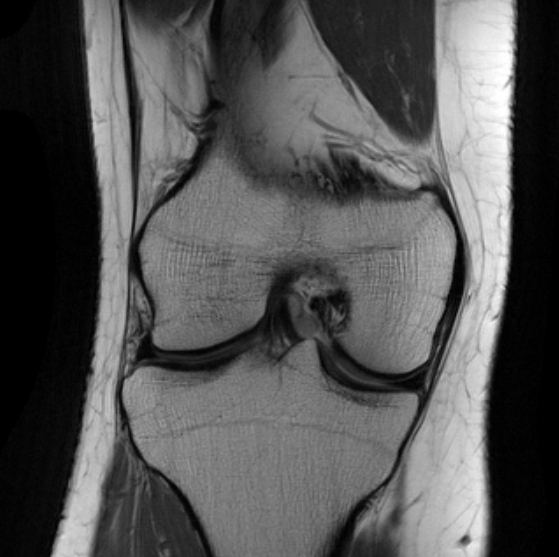
\includegraphics[width=\textwidth]{figs/ref.png}
   \caption{원래 이미지, $x$}
  \end{subfigure}
  \begin{subfigure}[b]{0.3\textwidth}
   \centering
   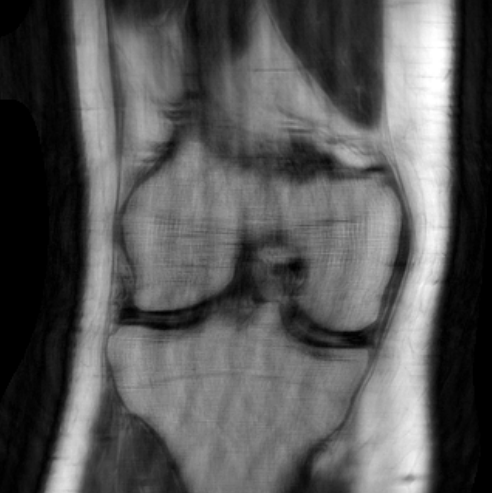
\includegraphics[width=\textwidth]{figs/zero.png}
   \caption{zero-filled 이미지, $x_{zero}$}
  \end{subfigure}
  \begin{subfigure}[b]{0.3\textwidth}
   \centering
   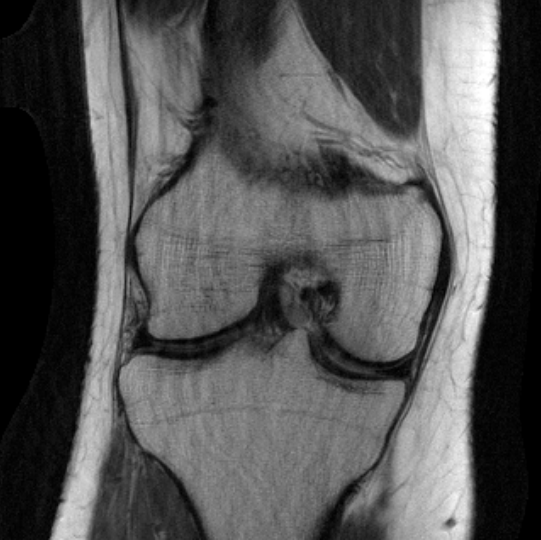
\includegraphics[width=\textwidth]{figs/sense.png}
   \caption{CS 를 통해 복원된 이미지 $\hat{x}$}
  \end{subfigure}
  \caption{예시 구현 결과물}\label{fig:results}
\end{figure}

구현의 결과물은 \figref{fig:results} 와 같이 $x_{zero}$ 는 선명하지 못한데 반해 CS 로 복원한 $\hat{x}$ 는 상대적으로 더 디테일이 잘 보이도록 나와야 한다. $x$ 에 비해 $\hat{x}$ 가 선명하지 않거나 두 영상이 어느 정도 차이를 보이는 것은 CS 의 한계로 인한 것이다.

\end{document}
